\documentclass[11pt,a4paper]{article}
\usepackage[utf8]{inputenc}
\usepackage[T1]{fontenc}
\usepackage{lmodern}
\usepackage[margin=2.5cm]{geometry}
\usepackage{xcolor}
\usepackage{titlesec}
\usepackage{hyperref}
\usepackage{graphicx}
\usepackage{listings}
\usepackage{tabularray}
\usepackage{tcolorbox}
\usepackage{enumitem}
\usepackage{fancyhdr}
\usepackage{lastpage}

% Color definitions
\definecolor{primaryColor}{RGB}{34, 45, 101}
\definecolor{secondaryColor}{RGB}{46, 117, 182}
\definecolor{accentColor}{RGB}{255, 87, 34}

% Hyperref setup
\hypersetup{
    colorlinks=true,
    linkcolor=primaryColor,
    filecolor=secondaryColor,
    urlcolor=accentColor,
    pdftitle={Data Analysis Project},
    pdfauthor={Your Name},
}

% Section formatting
\titleformat{\section}
  {\color{primaryColor}\Huge\bfseries}
  {\thesection}{1em}{}

\titleformat{\subsection}
  {\color{secondaryColor}\Large\bfseries}
  {\thesubsection}{1em}{}

% Page style
\pagestyle{fancy}
\fancyhf{}
\fancyhead[L]{\textit{Data Analysis Project}}
\fancyhead[R]{\thepage\ of \pageref{LastPage}}
\fancyfoot[C]{\textcolor{primaryColor}{\rule{0.8\textwidth}{0.4pt}}}

% Code listing style
\lstdefinestyle{customcode}{
    backgroundcolor=\color{gray!10},
    commentstyle=\color{green!60!black},
    keywordstyle=\color{blue},
    stringstyle=\color{orange},
    basicstyle=\ttfamily\footnotesize,
    breakatwhitespace=false,
    breaklines=true,
    captionpos=b,
    keepspaces=true,
    numbers=left,
    numbersep=5pt,
    showspaces=false,
    showstringspaces=false,
    showtabs=false,
    tabsize=2
}
\lstset{style=customcode}

\definecolor{dkgreen}{rgb}{0,0.6,0}
\definecolor{gray}{rgb}{0.5,0.5,0.5}
\definecolor{mauve}{rgb}{0.58,0,0.82}

\lstset{frame=tb,
  language=Python,
  aboveskip=3mm,
  belowskip=3mm,
  showstringspaces=false,
  columns=flexible,
  basicstyle={\small\ttfamily},
  numbers=none,
  numberstyle=\tiny\color{gray},
  keywordstyle=\color{blue},
  commentstyle=\color{dkgreen},
  stringstyle=\color{mauve},
  breaklines=true,
  breakatwhitespace=true,
  tabsize=3
}

%  make besutiful and styled tcolorbox for response for the prompts
\newtcolorbox{responsebox}{
    colback=gray!5,
    colframe=gray!50!black,
    breakable
}


\begin{document}

\begin{titlepage}
\centering
{\Huge\bfseries Data Analysis Project\par}
\vspace{2cm}
{\Large\itshape Ayush Kumar Mishra\par}
\vfill
{\large \today\par}
\end{titlepage}

\tableofcontents

\newpage

\section{Introduction}
\label{sec:intro}
This document outlines the process of using ChatGPT to generate prompts for results and analysis of the project, extracted from the data.

\subsection{Outline of the Document}
\begin{itemize}[leftmargin=*]
    \item Prompts used for data analysis
    \item Prompts used for Streamlit Dashboard
    \item Prompts used for project results
    \item Prompts used for LaTeX writing
\end{itemize}

\section{Data Overview}
\label{sec:data-overview}

\textbf{Primary Prompt:} "What types of data were analyzed (emotion, gaze, and transcript data)? Can you explain the key features like emotion categories, gaze measurements, and transcript sentiments?"

\textbf{Follow-up Prompts:}
\begin{itemize}[leftmargin=*]
    \item "Can you explain the structure of the gaze data, such as blink and eye offset values?"
    \item "What are the basic statistics for the transcript data?"
\end{itemize}

\section{Data Preprocessing}
\label{sec:preprocessing}

\textbf{Prompt:} "What preprocessing steps were applied to the data, including handling missing values, encoding categorical features, and scaling or normalization?"


\newpage
\section{Data Preparation and Integration}
\label{sec:data-prep}

In this section, I explain how the data was prepared and important features were extracted from the three provided CSV files.

\subsection{Extracting Key Features from Emotion Data from each CSV file and making single DATAFRAME}
\textbf{Initial Prompt:}
\begin{tcolorbox}[breakable, colback=gray!5, colframe=gray!50!black]
\lstinputlisting[language=Python]{prompts/emotion_prompt.txt}
\end{tcolorbox}
\begin{center}
    \color{red}\rule{1\linewidth}{0.5mm}
\end{center}


\begin{responsebox}
    Chatpgt gave wrong response to the initial prompt. The response was giving wrong results.\\
    So i further explained what i intended to do
\end{responsebox}
   



\textbf{Refined Prompt:}
\begin{verbatim}
You are doing it incorrectly. I want to first calculate the most frequent 
of every single emotion CSV and then make one column out of it. 
Then, finally make 10 columns out of 10 CSV files with column names 
dominat\_top1, dominant\_top2 emotions. From every emotion CSV, find 
2 max frequency dominant features and then add that.
\end{verbatim}
\begin{center}
    \color{red}\rule{1\linewidth}{0.5mm}
\end{center}


\textbf{For this prompt, response from the chatgpt was:}
\begin{tcolorbox}[breakable, colback=gray!5, colframe=gray!50!black]
\lstinputlisting[language=Python]{prompts/code1.txt}
\end{tcolorbox}

\large{With the help of this code, two most freq dominant emotions were extracted from each emotion CSV file and added to the final dataframe.\\}

\large{

Now the final dataframe has 10 columns with features top\_1\_dominant, top\_2\_dominant emotion.}
\begin{center}
    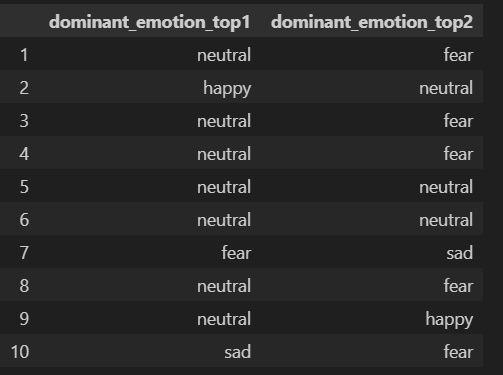
\includegraphics[width=1\columnwidth]{images_prompts/dominant_emotion.png}
\end{center}

\subsection{Integrating transcript data with emotion data}

\textbf{Prompt:}
\begin{tcolorbox}
    \lstinputlisting[language=Python]{prompts/trans_promt.txt}
\end{tcolorbox}
\begin{center}
    \color{red}\rule{1\linewidth}{0.5mm}
\end{center}

\begin{responsebox}
    The response from the chatgpt awesome this time.
\end{responsebox}

\begin{tcolorbox}
    \lstinputlisting[language=Python]{prompts/code2.txt}
\end{tcolorbox}

\large{Using above code, It extracted the above features of transcript data of each student and added to the final dataframe.}
\begin{center}
    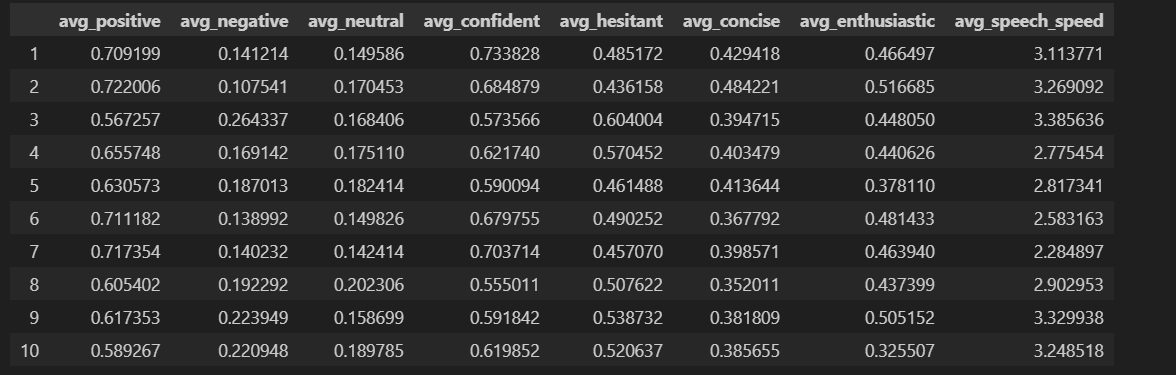
\includegraphics[width=1\columnwidth]{images_prompts/trans_df.png}
\end{center}

\begin{tcolorbox}[colback=yellow!10!white, colframe=red!80!black, title=Note]
  Now we have to merge the transcript data with the emotion data. \\
  For that we have to merge the dataframes on the basis of student id.
\end{tcolorbox}

\textbf{Prompt for merging the emotion\_df and transcript\_df:}
\begin{verbatim}
    df_dominantEmotion_for_everystudent
    and final_df add these df on index
\end{verbatim}
\begin{center}
    \color{red}\rule{1\linewidth}{0.5mm}
\end{center}

\text{response from the chatgpt:}
\begin{tcolorbox}
\begin{lstlisting}
final_df_with_emotions = pd.concat([final_df, df_dominantEmotion_for_everystudent], axis=1)

# Print the final merged DataFrame
print(final_df_with_emotions.head(10))

\end{lstlisting}
\end{tcolorbox}

\large{Using the above code, the emotion data and transcript data were merged on the basis of student id.}
\large{The final dataframe after merging the emotion and transcript data is shown below:}

\begin{tcolorbox}[colback=blue!5!white, colframe=green!70!black, title=Final Dataframe, fonttitle=\bfseries\Large]
\begin{tblr}{
    colspec = {lccccccccccc},
    row{1} = {font=\bfseries\color{red}},
    hlines,
    vlines,
    stretch = 0.1
}
\textbf{id} & \textbf{avg\_positive} & \textbf{avg\_negative} & \textbf{avg\_neutral} & \textbf{avg\_confident}  \\
1 & \textcolor{blue}{0.709199} & \textcolor{blue}{0.141214} & \textcolor{blue}{0.149586} & 0.733828 \\
2 & \textcolor{blue}{0.722006} & \textcolor{blue}{0.107541} & \textcolor{blue}{0.170453} & 0.684879 \\
\end{tblr}

\begin{tblr}{ colspec = {lccccccccccc},
    row{1} = {font=\bfseries\color{red}},
    hlines,
    vlines,
    stretch = 1}
\textbf{avg\_hesitant} & \textbf{avg\_concise} & \textbf{avg\_enthusiastic} & \textbf{avg\_speech\_speed} \\
0.485172 & 0.429418 & 0.466497 & 3.113771  \\
 0.436158 & 0.484221 & 0.516685 & 3.269092 \\
\end{tblr}
\begin{tblr}{ colspec = {lccccccccccc},
    row{1} = {font=\bfseries\color{red}},
    hlines,
    vlines,
    stretch = 1}

\textbf{dominant\_emotion\_top1} & \textbf{dominant\_emotion\_top2} \\
neutral & fear \\
happy & neutral \\
\end{tblr}
\end{tcolorbox}

\section{Prompts for Analysis on the DataFrame made above}

\subsection{Basic Statistics}
\textbf{Prompt:}
\begin{tcolorbox}
    \begin{lstlisting}
     How to know whether there are any missing values in the final DataFrame?
     or just give me description of the dataframe.
    \end{lstlisting}
\end{tcolorbox}

\textbf{Response:}
\begin{tcolorbox}
    \begin{lstlisting}
    print(final_df_with_emotions.describe())
    \end{lstlisting}
\end{tcolorbox}

\large{The basic statistics of the final DataFrame are as follows:}
\begin{center}
    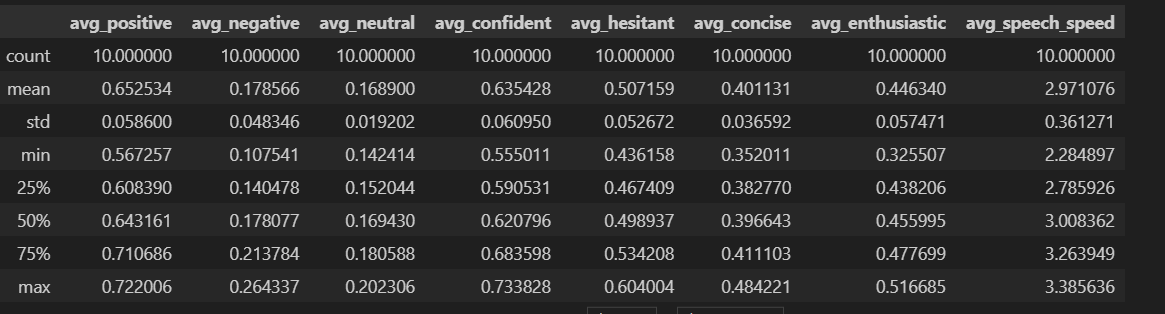
\includegraphics[width=1\columnwidth]{images_prompts/basic-stats.png}
\end{center}


\subsection{Correlation Analysis}
    Now i did correlation analysis on the final DataFrame to understand the relationship between different features.
\textbf{Prompt:}
\begin{tcolorbox}
    \begin{lstlisting}
    Now, calculate the correlation matrix of the final DataFrame final\_df.
\end{lstlisting}
\end{tcolorbox}

\textbf{Response:}
\begin{tcolorbox}
    \begin{lstlisting}
    correlation_matrix = final_df_with_emotions.corr()
    print(correlation_matrix)
    \end{lstlisting}
\end{tcolorbox}

\large{Wrtitng and running the code, there was a error in chatgpt response, but 
I corrected it and ran the code. The correlation matrix is shown below:}

\begin{center}
    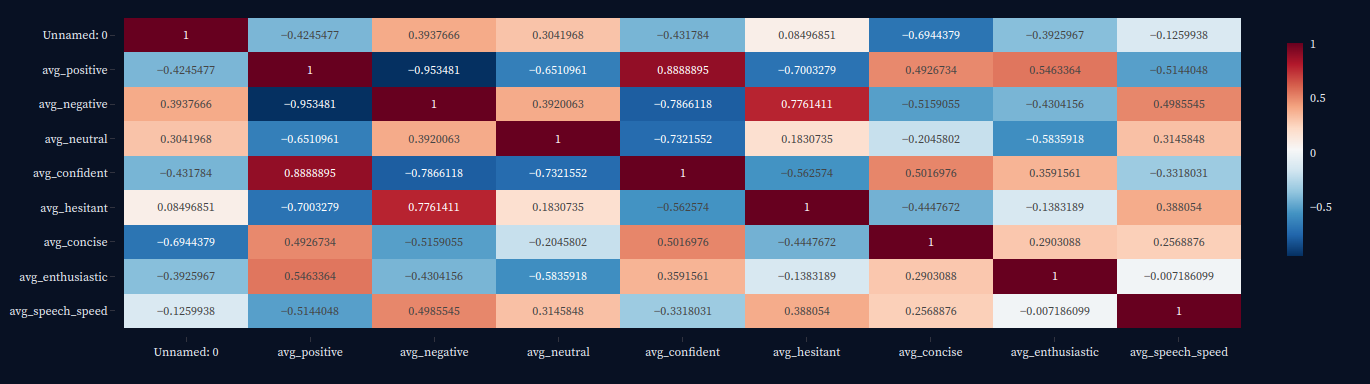
\includegraphics[width=1\columnwidth]{images/corr.png}
\end{center}

\subsection{Based on the final\_df, I asked for analysis on the data.}
\textbf{Prompt:}
\begin{tcolorbox}
  \lstinputlisting[language= python]{prompts/main.txt}
\end{tcolorbox}

\textbf{Response:}
\begin{tcolorbox}
    \lstinputlisting{prompts/main-res.txt}
  \end{tcolorbox}
  


% Additional sections continue in a similar format...

\section{Conclusion}
\label{sec:conclusion}
This section summarizes the key findings and insights from the data analysis project.

% References
\bibliographystyle{plain}
\bibliography{references}

\end{document}